\documentclass{article}
\usepackage{amsmath}
\usepackage[utf8]{inputenc}
\usepackage{graphicx}
\setlength{\parskip}{\baselineskip}%
\setlength{\parindent}{0pt}%

\begin{document}
\title{Veckotest 1}
\author{Henrik Samuelsson}
\maketitle
\textbf{1.} Lös ekvationen $7x-2(3x-8)=45$

\textbf{Lösning}\\
$7x-2(3x-8)=45$\\
$7x-6x+16=45$\\
$7x-6x=45-16$\\
$x=29$

\textbf{2.} Låt $f(x)=4x^{2}+2x$ och bestäm\\
\textbf{a)} $f(0)$\\
\textbf{b)} $f(3)$\\
\textbf{c)} $f(-1)$\\
\textbf{d)} $f(2a + 3a)$

\textbf{Lösning}\\
\textbf{a)} $f(0)=4\cdot0^2+2\cdot0=4\cdot0=0$\\
\textbf{b)} $f(3)=4\cdot3^2+2\cdot3=4\cdot9+4=36+4=40$\\
\textbf{c)} $f(-1)=4(-1)^2+2(-1)=4\cdot1-2=4-2=2$\\
\textbf{d)} $f(2a+3a)=4\cdot(2a+3a)^2+2\cdot(2a+3a)=4(4a^2+12a+9a^2)+10a=52a^2+58a$

\textbf{3.} En linje är parallell med linjen $2x - y = 0$ och går genom punkten $(4, -1)$. Bestäm linjens ekvation.

\textbf{Lösning}\\
Den kända linjen kan skrivas som $y = 2x$.

Den sökta linjen är parallell med den kända linjen, det betyder att den sökta linjen måste kunna skrivas som $y = 2x + m$.

Vi känner inte till värdet av $m$ men kan få fram det eftersom vi känner till en punkt på den sökta linjen. Vi sätter in koordinaterna för den kända punkten i linjens ekvation.

$-1 = 2 \cdot 4 + m$\\
$-1 = 8 + m$\\
$m = -1 - 8$\\
$m = -9$

Den sökta linjens ekvation är således $y = 2x - 9$.

Som en extra kontroll kan man plotta dom två linjerna. I bilden nedan ser vi dom två linjerna. Resultatet verkar rimligt, linjerna ser parallella ut och en av linjerna gå igenom den givna punkten. 

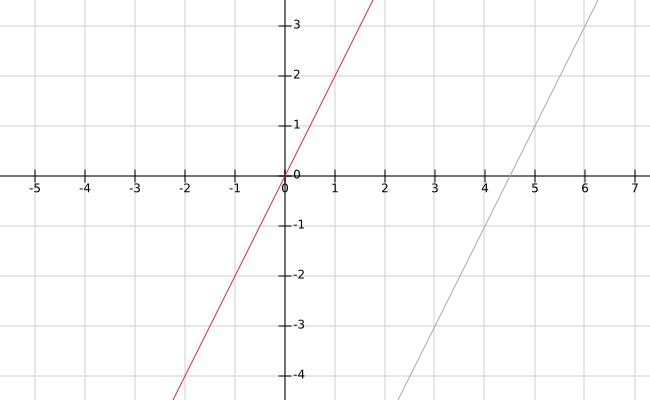
\includegraphics[scale=0.65]{graph_1_3_1.png} 

\textbf{4.} Ange ekvationen för en linje som är vinkelrät mot linjen $y=\dfrac{x}{3}-7$.

\textbf{Lösning}\\
I kurslitteraturen bevisas att två icke-vertikala linjer med riktningskoefficienterna $k_{1}$ och $k_{2}$ är vinkelräta om och endast om $k_{2} = -\dfrac{1}{k_{1}}$.

Vi har en given linje med riktningskoefficienten $k_{1} = \dfrac{1}{3}$. Det betyder att att en linje som är vinkelrät mot den givna linjen måste ha  riktningskoefficienten $k_{2}=-3$.

Den sökta linjens m-värde kan väljas godtyckligt. Vi väljer $m = 3$.

Ekvationen för den sökta linjen blir $y = -3x + 3$.

Som en extra kontroll väljer vi även att plotta ut dom två linjerna. I bilden nedan ser vi dom två linjerna. Linjerna ser hyfsat vinkelräta ut så vi har antagligen räknat rätt.

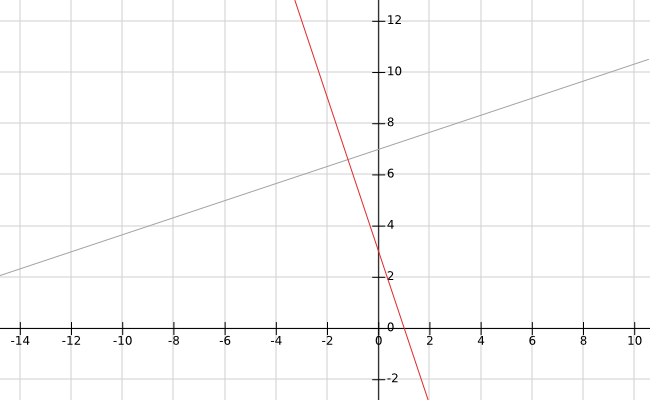
\includegraphics[scale=0.65]{graph_1_4_1.png}

\end{document}
